\chapter[برخی نکات مفید]{ برخی نکات مفید ( اضافه کردن عنوان برای بیش از یک خط شدن)}
\twocolumnfootnotes
\section{فرایند تصویب پیشنهادیۀ پارسای تحصیلات تکمیلی}
در این بخش، فرآیند تصویب پیشنهادیۀ پایان‌نامه/رساله آورده شده است. 
دستورالعمل کامل مراحل تصویب و ثبت پیشنهادیۀ پایان‌نامه/ رساله دانشجویان تحصیلات تکمیلی در پیوست~\ref{ch:proposal}
آمده است.

لطفا برای مشاهده آخرین تغییرات به وبسایت تحصیلات تکمیلی دانشگاه به آدرس

\centerline{\url{https://yazd.ac.ir/offices/educational/deputy/graduate/home/rules}}

مراجعه نمایید.

\centerline{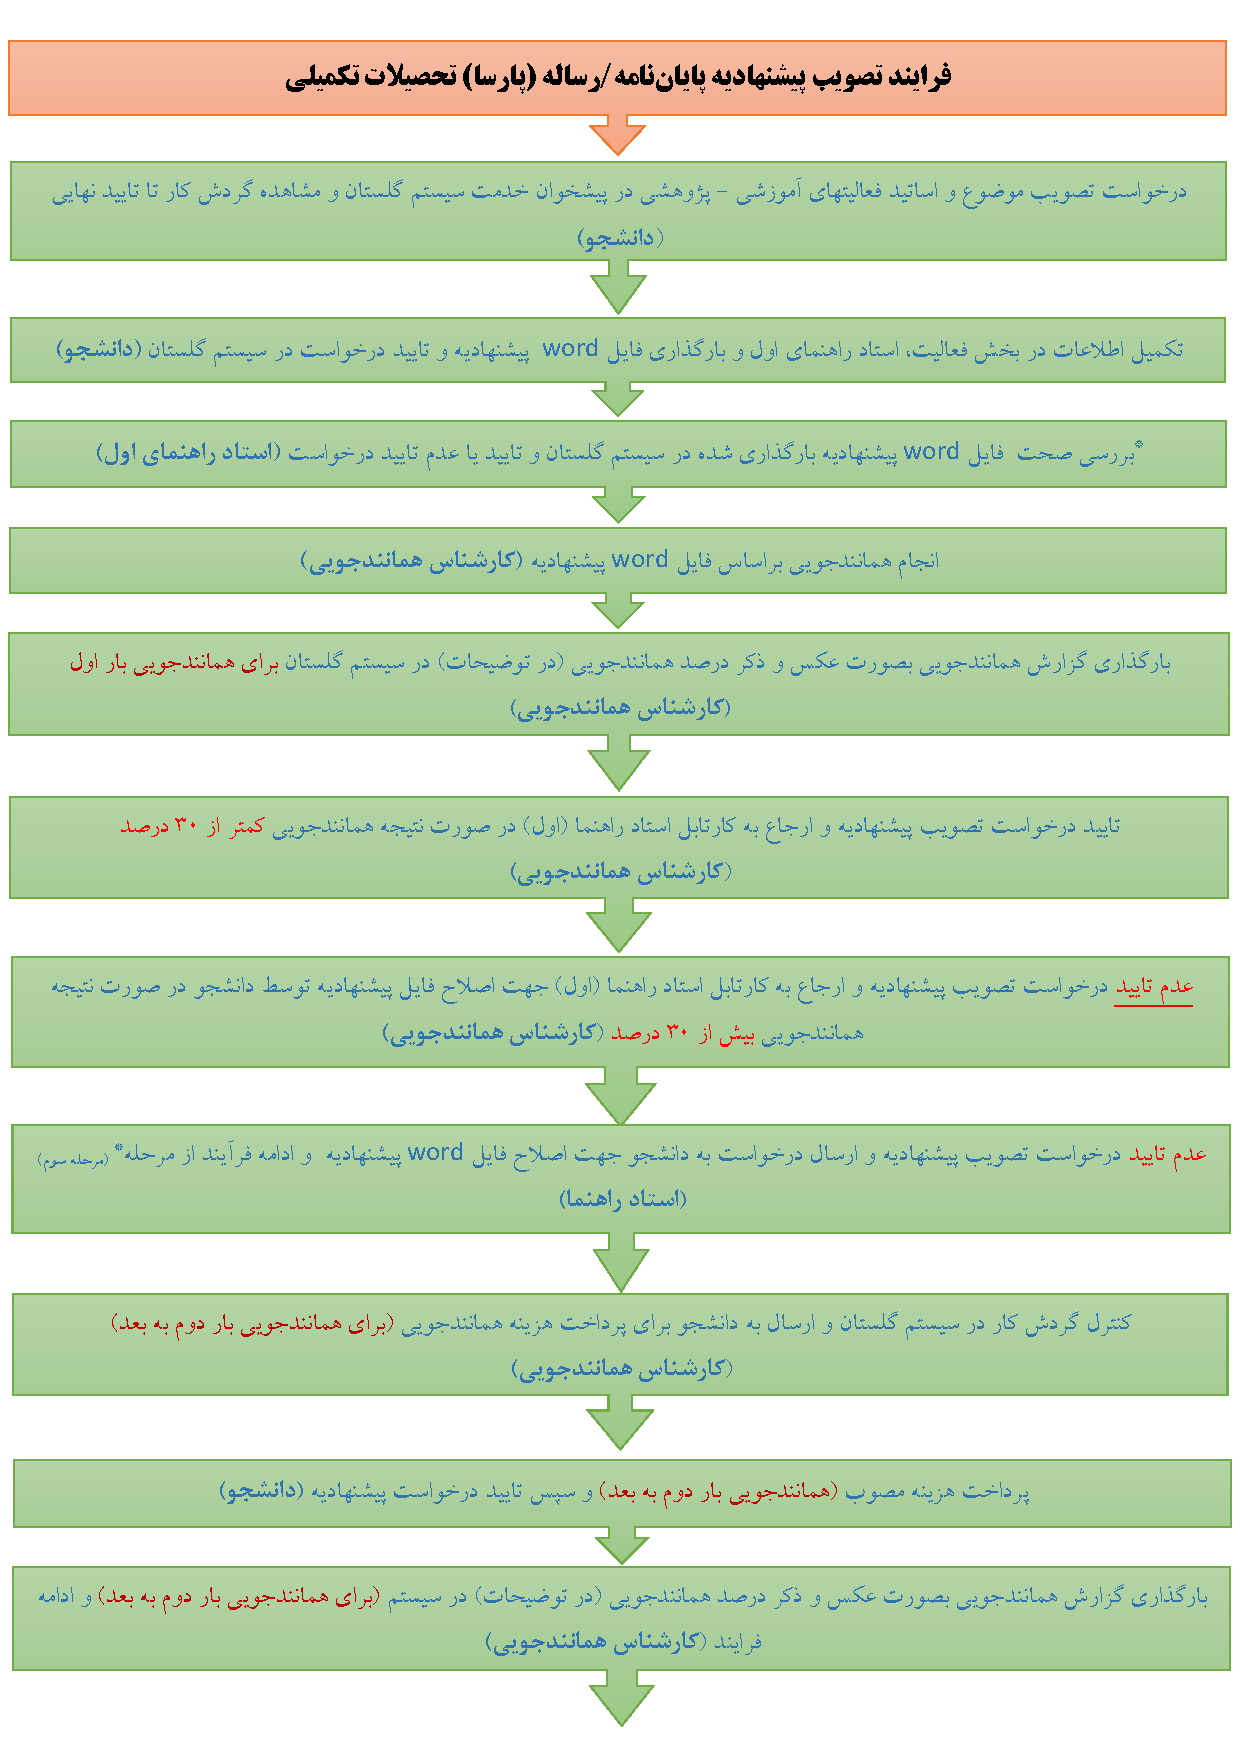
\includegraphics[width=0.9\textwidth]{Proposal-chart_Part1}}

\centerline{\includegraphics[width=\textwidth]{Proposal-chart_Part2}}

\section{دستورالعمل نحوه برگزاری جلسات دفاع }
\subsection{هدف }
هدف از تدوین این دستورالعمل ایجاد نظم و ترتیب بیشتر و شفاف‌سازی چگونگی برگزاری جلسات دفاع پایان‌نامه 
کارشناسی ارشد و رساله دکتری  و یادآوری نکات مهم برای برگزاری جلسه مطابق مقررات و شیوه‌نامه‌های تحصیلات تکمیلی‌است 
که بر اساس صورتجلسه شورای تحصیلات تکمیلی دانشگاه مورخ 17/2/1397 توسط نماینده تحصیلات تکمیلی (ناظر جلسه دفاعیه) 
دانشگاه مدیریت می‌گردد. 

\subsection{الف) فرآیند دفاع از پایان‌نامه / رساله }

\begin{enumerate}
\item  دانشجو: درخواست دفاع در پیشخوان خدمت

دانشجو در این قسمت ضمن درخواست دفاع‏، تاریخ و محل پیشنهادی دفاع از پایان‌نامه / رساله را بر اساس هماهنگی به عمل آمده
 با استادان راهنما / مشاور و پس از تایید اولیه رئیس بخش/ مدیرگروه ثبت می‌نماید. 
برای این منظور لازم است: 

*‌ دانشجو ظرف 48 ساعت، پایان‌نامه / رساله خود را همراه با مقالات مستخرج و تأییدیه‌های مجلات برای طرح در شورا به
 رئیس بخش / مدیرگروه تحویل و پس از تصویب جزئیات دفاع در شورا، فایل پایان‌نامه / رساله تصحیح شده نهایی و دستاوردهای
 مستخرج از آن را برای كارشناس تحصیلات تكمیلی ارسال کرده و فرآیند دفاع را تا مرحله تأیید معاون دانشكده / مدیرگروه مستقل پیگیری می‌نماید. 
 
*‌ برای دانشجویان دکتری لازم است كاربرگ بررسی مقالات از قبل با رعایت ضوابط مربوط تأیید و جلسه پیش دفاع دانشجو
 (حداقل 21 روز قبل از تاریخ دفاع) مطابق مقررات به طور موفقیت‌آمیز برگزار شده باشد و کاربرگ‌های مربوطه تکمیل، تایید و 
 به کارشناس جهت ثبت و بارگذاری در سیستم گلستان تحویل شده باشد.

\item  دانشجو: انجام نظرسنجی 

در این مرحله دانشجو باید نظرسنجی از استادان راهنما و مشاور پایان‌نامه / رساله را انجام و تایید نماید. 

\item  دانشجو: ضمیمه کردن همزمان فایل‌های word و  pdfپایان‌نامه / رساله

در این مرحله دانشجو فایل تصحیح شده نهایی پایان‌نامه / رساله را پیوست و برای انجام فرآیند همانندجویی ارسال می‌نماید. 
لازم به ذکر است فایل pdf  ضمیمه شده همان فایلی است که در اختیار اعضای هیأت داوران قرار می‌گیرد. 

* ضروری است تنها در نسخه word پایان نامه مفاد دستورالعمل بارگذاری رساله/پایان نامه برای همانندجویی رعایت شده باشد.

* هزینه همانندجویی برای مرحله اول به عهده دانشگاه و در سایر مراحل به عهده دانشجو است. 

\item  استاد راهنما: بررسی صحت  فایل پایان‌نامه / رساله بارگذاری شده 

در این مرحله استاد راهنما (اول) فایل پایان‌نامه / رساله بارگذاری شده توسط دانشجو را مشاهده، کنترل و در صورت عدم مغایرت، 
درخواست دفاع را تایید می‌نماید، در غیر اینصورت بایستی با انتخاب گزینه «عدم تایید» درخواست دفاع به کارتابل دانشجو عودت شود
 و دانشجو نسبت به انجام اصلاحات و بارگذاری فایل صحیح پایان‌نامه / رساله مجدداً اقدام نماید. 

\item  کارشناس همانندجویی دانشکده / گروه مستقل: انجام همانندجویی 

5-1- همانندجویی برای بار اول

کارشناس همانندجویی دانشکده / گروه مستقل، متن فایل word پیوست شده توسط دانشجو را در سامانه همانندجویی کپی 
و ارسال و نتیجه را در فایل دانشجو بارگذاری و درخواست را (با ذکر درصد همانندی در توضیحات) تایید / عدم تایید می‌نماید. 
*در صورتی که نتیجه همانندجویی کمتر از 30 درصد باشد، درخواست دفاع دانشجو تایید و به کارتابل استاد راهنما جهت طی 
مراحل بعدی ارجاع می‌شود. 

*در صورتی که نتیجه همانندجویی بیشتر از 30 درصد باشد، درخواست دفاع دانشجو عدم تایید و جهت اصلاح پایان‌نامه / رساله توسط دانشجو، 
به کارتابل استاد راهنما برمی‌گردد. 

5-2- همانندجویی برای بار دوم به بعد

*در صورتی که همانندجویی برای بار دوم به بعد انجام می‌شود (با کنترل گردش کار در گلستان)، کارشناس درخواست دفاع را برای 
پرداخت هزینه همانندجویی به دانشجو ارسال می‌‌نماید. 

5-2-1- دانشجو: پرداخت هزینه همانندجویی بار دوم به بعد

در صورتی که همانندجویی برای بار دوم به بعد انجام می‌شود دانشجو ملزم به پرداخت هزینه مصوب و تایید درخواست دفاع است. 

5-2-2- کارشناس همانندجویی دانشکده / گروه مستقل

 بعد از پرداخت هزینه توسط دانشجو فرآیند همانندجویی مطابق  بخش 5-1- انجام و ادامه می‌یابد. 

\item  استاد راهنما

در این مرحله استاد راهنما (اول) نتیجه همانندجویی را مشاهده می‌کند. در صورت همانندی کمتر از 30 درصد، درخواست دفاع 
تایید و برای استاد راهنمای دوم / مشاور ارسال می‌شود، در صورت همانندی بیش از 30 درصد گزینه عدم تایید انتخاب و نتیجه 
به دانشجو ارجاع می‌گردد. در این مرحله دانشجو ملزم به اصلاح پایان‌نامه / رساله  براساس گزارش همانندجویی با نظارت استاد راهنما
 و ادامه روند از مرحله 3 است. 

\item استاد راهنمای دوم/ استاد(ان) مشاور

در این مرحله استاد راهنمای دوم / استاد(ان) مشاور فایل پایان‌نامه / رساله و نتیجه همانندجویی را مشاهده و درخواست دفاع را تأیید یا عدم تایید می‌نماید.

\item  رئیس بخش/ مدیرگروه

در این مرحله رئیس بخش/ مدیر گروه درخواست دفاع تأیید شده توسط استادان راهنما و مشاور را همراه با پایان‌نامه / رساله 
بارگذاری شده به همراه نتیجه همانندجویی در جلسة شورای بخش/گروه مطرح می‌نماید. پس از تایید پایان نامه/رساله و مستندات 
و انطباق فایل مذکور با پیشنهادیه تصویب شده، استادان داور در این جلسه تعیین و سپس تاریخ، نام استادان داور و محل برگزاری 
دفاع در سیستم گلستان توسط رئیس بخش / مدیرگروه ثبت می‌شود. 

*‌ نکته 1: استادان داور خارج از دانشگاه، بدون کد استادی و استادان داخل دانشگاه با کد استادی فعال تعریف می‌شوند. 

*‌ نکته 2: رئیس بخش / مدیر گروه می‌تواند پس از تأیید  با استفاده از گزارش 6822 سیستم گلستان دعوت‌نامه استادان راهنما، 
مشاور و داوران را دریافت نماید و به آنها تحویل دهد.

\item  کارشناس تحصیلات تکمیلی پردیس / دانشکده مستقل:

کارشناس تحصیلات تکمیلی پردیس / دانشکده مستقل پرونده دانشجو را از لحاظ آموزشی (حذف سرترم اضافی، ایجاد سرترم مورد نیاز، بررسی
 فرم‌های گزارش پیشرفت و...)، موجود بودن مستندات پژوهشی قبل از دفاع نظیر فرم بررسی مقالات، صورتجلسه پیش دفاع و ... در پرونده
 و سامانه گلستان بررسی و سپس درخواست مذکور را تایید می‌نماید. 
 
*در صورت بدهکار بودن دانشجو، درخواست دفاع بعد از تایید کارشناس به کارتابل دانشجوی بدهکار ارجاع می‌شود. دانشجو موظف است 
نسبت به پرداخت بدهی در سیستم گلستان اقدام و درخواست دفاع را مجدداً تایید نماید. 

\item  استادان داور: 

در این مرحله داوران پس از مشاهده و اخذ فایل پایان‌نامه / رساله بارگذاری شده در گلستان و نتیجه همانندجویی، درخواست دفاع را تأیید / عدم تایید
 می‌نمایند. 

\item  معاون آموزشی دانشکده/مدیر گروه مستقل:

در این مرحله معاون دانشکده/ مدیر گروه مستقل پس از مشاهده پایان‌نامه / رساله بارگذاری شده در گلستان و نتیجه همانندجویی 
درخواست دفاع دانشجو را تأیید (با رعایت فاصله زمانی دفاع)/ عدم تایید می‌نماید.

*‌ نکته1: توصیه می‌شود فایل تایید شده در شورای بخش/گروه به همراه سایر مستندات مجدداً در شورای دانشکده/گروه مستقل بررسی
 و با ضوابط تحصیلات تکمیلی مطابقت داده شود. تائید معاون دانشکده/ مدیر گروه مستقل به منزله تایید علمی پایان‌نامه/رساله از سوی 
 شورای دانشکده/گروه مستقل است.
 
* نکته2: چک کردن مستندات بارگذاری شده پیش دفاع برای دانشجویان دکتری الزامی است.

*‌ نکته 3: رعایت زمان 10 روزه برای دانشجویان ارشد و 15 روزه برای دانشجویان دکتری، از زمان تأیید معاون دانشکده / مدیر گروه مستقل الزامی است. 


\item  کارشناس حوزه تحصیلات تکمیلی: تعیین ناظر

دراین قسمت حوزه تحصیلات تکمیلی ناظر جلسه دفاع را تعیین و نام ایشان را در قسمت فعالیت‌های دانشجو درج می نماید.  

\item  کارشناس تحصیلات تکمیلی پردیس / دانشکده مستقل

کارشناس تحصیلات تکمیلی گزارش‌ها و مستندات لازم را اخذ و همراه فرم‌های مربوط به دفاع برای استاد ناظر ارسال می‌نماید. 

\item  برگزاری جلسه دفاع در زمان و مکان مقرر
\end{enumerate}


**توجه: دانشجویان موظف هستند با مراجعه به پیشخوان خدمت و مشاهده گردش کار، از وضعیت درخواست خود
 اطلاع حاصل نمایند و در صورت تایید نهایی از گزارش 1567 اطلاعیه دفاع را پرینت گرفته و ضمن اطلاع رسانی برای برگزاری 
 جلسه دفاع در سایت دانشکده/گروه مستقل، پس از مطالعه دستورالعمل شرایط و نحوه برگزاری جلسات دفاع، در زمان و مکان مقرر اقدام نمایند.

\subsection{ب) نکات قابل توجه در انجام فرایند دفاع قبل، حین و بعد از جلسه دفاع}

*‌ دانشجویان دکتری بایستی قبل از درخواست دفاع، امور مربوط به برگزاری جلسه پیش دفاع را مطابق با دستورالعمل مربوط انجام دهند. 

*‌ دانشجو پس از اخذ مجوز دفاع (تایید معاون دانشکده / مدیرگروه مستقل)، موظف است هماهنگی‌های لازم با استادان راهنما،
 مشاور و داوران جهت حضور در جلسه دفاع را به عمل آورد. 
 
*‌ درخواست دفاع، بعد از مطالعه شرایط و نحوه برگزاری جلسات دفاع و مطالعه دیگر شیوه‌نامه‌های تحصیلات تکمیلی، 
باید حداقل 4 هفته قبل از برگزاری جلسه دفاع توسط دانشجو در سیستم گلستان ثبت گردد. 

*‌ دانشجو موظف است پیگیری های لازم برای تأیید درخواست دفاع در سیستم گلستان تا آخرین مرحله تأیید را به عمل آورد. 

*‌ شرایط داوران پیشنهادی و استفاده از شرایط ویدئوکنفرانس بایستی مطابق با شیوه‌نامه‌های تحصیلات تکمیلی دانشگاه موجود در وب‌سایت دانشگاه باشد.

*‌ رعایت زمان 10 روزه برای دانشجویان کارشناسی ارشد و 15 روزه برای دانشجویان دکتری از زمان تأیید معاون دانشکده / مدیر گروه مستقل، 
در سیستم گلستان الزامی است.

*‌ اطلاع رسانی عمومی دفاع (پرینت نسخه از سایت از گزارش 1567 گلستان) با درج اطلاعیه در وب‌سایت دانشکده / گروه مستقل 
و تابلوی اعلانات توسط دانشجو با هماهنگی بخش / گروه حداقل یک هفته قبل از برگزاری جلسه دفاع الزامی است.

*‌ بعد از تعیین تاریخ دفاع، امکان لغو یا تغییر تاریخ وجود ندارد. 

*‌ در تعیین زمان دفاع توسط رئیس بخش / مدیرگروه هنگام تعریف بازه زمانی، لازم است زمان پایان دفاع یک دقیقه کمتر درج گردد 
بعنوان مثال زمان دفاع بجای 10-8 بصورت 9:59 -8 درج گردد. 

*‌ عنوان پایان نامه / رساله دانشجو با عنوان ذکر شده در فرم تصویب پیشنهادیه بایستی یکسان باشد. در صورت اصلاح عنوان در جلسه 
دفاع لازم است کاربرگ مربوط تکمیل و تأیید و به ناظر تحصیلات تکمیلی تحویل داده شود. 

*‌ رئیس بخش / مدیر گروه می‌تواند پس از تأیید  با استفاده از گزارش 6822 سیستم گلستان دعوت‌نامه استادان راهنما، مشاور و 
داوران را دریافت نماید و به آنها تحویل دهد. 

*‌ مدت زمان ارائه پایان‌نامه توسط دانشجوی کارشناسی ارشد (حداقل 20 و حداکثر30 دقیقه) و مدت زمان برگزاری جلسه 
دفاع از پایان‌نامه کارشناسی ارشد (حداقل 60 و حداکثر120 دقیقه) است. 

*‌ مدت زمان ارائه توسط دانشجوی دکتری (حداقل 30 و حداکثر50 دقیقه) و مدت زمان برگزاری جلسۀ دفاعیه
 دکتری (حداقل 120 و حداکثر180 دقیقه) است. 
 
*‌ پس از برگزاری جلسه دفاع، دانشجو موظف است ضمن کنترل دقیق نگارش و فرمت پایان نامه / رساله، اصلاحات لازم را تا موعد 
مقرر زیر نظر استادان راهنما و مشاور انجام داده کاربرگ مربوط را تکمیل و تأییدیه‌های لازم را اخذ نماید. 

* دانشجو موظف است حداکثر 3 ماه بعد از برگزاری جلسه دفاع، کلیه امور مربوط به فارغ‌التحصیلی خود اعم از انجام اصلاحات، 
تحویل فایل الکترونیکی پایان‌نامه / رساله به استادان راهنما و مشاور، انجام تسویه و... انجام بدهد. در غیر این صورت مطابق با ضوابط مصوب
 دانشگاه با وی برخورد خواهد شد.  

\subsection{ج) دستورالعمل نحوه برگزاری جلسات دفاع: }
\begin{enumerate}
\item  برگزاری جلسه دفاع در تاریخ مقرر و تکمیل فرم‌های مربوط
\item  رعایت کلیه مفاد آیین‌نامه و مقررات جلسات دفاع از پایان‌نامه / رساله
\item 
 انجام پذیرایی (اختیاری) صرفاً در خارج محل برگزاری جلسه دفاع به منظور جلوگیری از ایجاد اختلال در نظم جلسه،
لازم است اقلام پذیرایی از هیأت داوران، دانشجویان و حضار دیگر در طی جلسه و هنگام ارائه مطالب دانشجو توزیع نشود 
و صرفاً در انتهای جلسه و در حد عرف انجام پذیرد. 
\item 
 اجتناب از دعوت و آوردن افراد خردسال و نوجوان 
\item 
 خودداری از قرار دادن گل و سایر تزئینات در جلسه دفاع
\item 
 خاموشی کامل یا گذاشتن در حالت بی‌صدا تلفن‌های همراه کلیه شرکت کنندگان و اعضاء هیأت داوران در طول جلسه. 
\item 
 تهیه فیلم (اختیاری) فقط در بخش ارائه جلسه دفاع (قبل از جلسه پرسش و پاسخ) و عکس‌برداری (اختیاری) منحصراً در مرحله 
ابراز قدردانی به گونه‌ای که موجب اختلال در برگزاری جلسه دفاع نگردد. 
\item 
 رعایت سایر موارد در جلسات دفاع مطابق با آخرین مقررات و مصوبات تحصیلات تکمیلی دانشگاه 
\end{enumerate}

\subsection{فرایند دفاع از پارسای تحصیلات تکمیلی}
در این بخش، فرآیند دفاع پایان‌نامه/رساله آورده شده است.  
 
لطفا برای مشاهده آخرین تغییرات به وبسایت تحصیلات تکمیلی دانشگاه به آدرس

\centerline{\url{https://yazd.ac.ir/offices/educational/deputy/graduate/home/rules}}

مراجعه نمایید.

\centerline{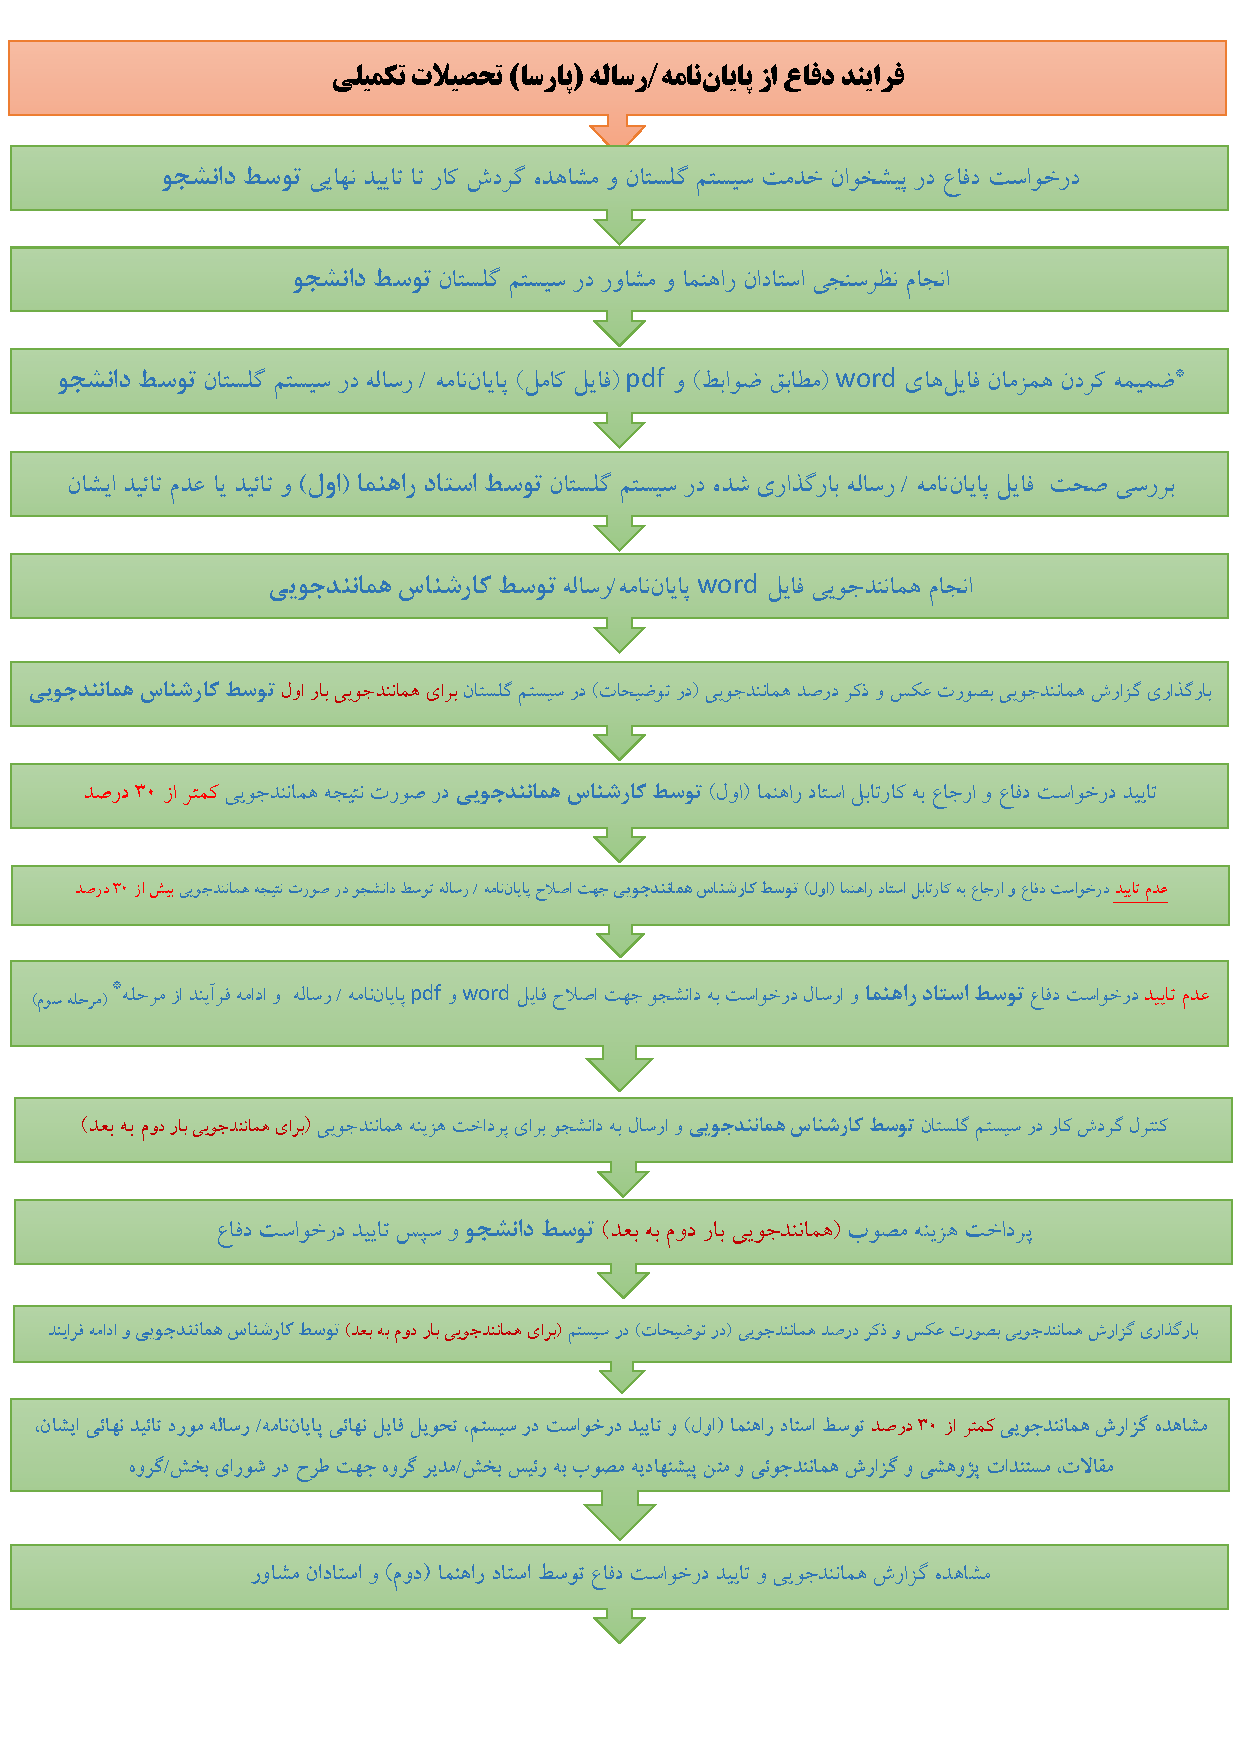
\includegraphics[width=0.95\textwidth]{defence-chart_Part1}}

\centerline{\includegraphics[width=\textwidth]{defence-chart_Part2}}

\section{توصیه‌های تحصیلات تکمیلی دانشگاه در خصوص پارساها}
این دستورالعمل به منظورآشنایی و آگاهی دانشجویان با نحوه نگارش و چگونگی تدوین و تنظیم مطالب یک تحقیق علمی (رساله) 
تهیه شده و ضروری است دانشجویان نکات مطرح شده در آن را هنگام تنظیم رساله رعایت نمایند.

\subsection{ بخش‌های رساله }

رساله باید مشتمل بر بخش‌های زیر باشد: 
\begin{enumerate}
\item شناسنامه یا صفحه عنوان (به زبان فارسی)
\item  شروع با ذکر نام خداوند
\item  صورت‌جلسه (فارسی) هیأت داوران جلسة دفاع از رساله 
\item  تعهدنامۀ رعایت حقوق معنوی دانشگاه یزد
\item  منشور اخلاق پژوهش
\item  تقدیم (اختیاری)
\item  سپاس و قدردانی (اختیاری)
\item  چکیده فارسی  
\item  فهرست مطالب
\item  فهرست شکل‌ها (در صورت داشتن شکل یا نمودار)
\item  فهرست جدول‌ها (در صورت داشتن جدول)
\item  فهرست نمادهای اختصاری و اختصارات (در صورت داشتن علائم، اختصارات و نمادهای اختصاری)
\item  پیشگفتار (اختیاری و با تصویب پردیس/دانشکده مستقل)
\item  متن اصلی که مشتمل بر فصل‌های مختلف از جمله مقدمه یا دیباچه، مروری بر منابع و مطالعات انجام شده و اهداف پژوهش، روش تحقیق، نتایج و تجزیه و تحلیل و تفسیر آنها، نتیجه‌گیری و پیشنهادها است. (مقدمه، فصل اول تلقی می‌شود.)
\item  واژه‌نامه فارسی به انگلیسی یا بالعکس (اختیاری و با تصویب پردیس/دانشکده مستقل و تایید شورای تحصیلات تکمیلی دانشگاه)
\item  فهرست منابع و مآخذ
\item  پیوست‌ها (در صورت وجود)
\item ABSTRACT (چکیده به زبان انگلیسی)
\item  شناسنامه یا صفحه عنوان (به زبان انگلیسی)
\end{enumerate}

\subsection{ حروف‌نگاری (تایپ) رساله}
\begin{enumerate}
 \item برای تایپ رساله از نرم‌افزار Word (نسخه 2013 یا بالاتر) یا LATEX استفاده شود و ترجیحاً متن اصلی با قلم 
BNazanin 14 (یا فونت مصوب پردیس/ دانشکده مستقل با تأیید شورای تحصیلات تکمیلی دانشگاه) باشد. 
متون انگلیسی با قلم \lr{Times New Roman 12} تایپ شود. برای تایپ رساله‌های رشتۀ ادبیات عرب ترجیحاً از قلم 
بدر عربی 15 استفاده شود.

\begin{center}
\begin{tabular}{|c|c|c|} \hline
نوع متن &	فونت فارسی	& فونت انگلیسی \\ \hline
متن عادی &	\lr{BNazanin 14}&	\lr{Times New Roman 12}\\ \hline
شماره صفحه‌ها	& \lr{BNazanin 12}	& \lr{Times New Roman 10}\\ \hline
عنوان فصل‌ها&	\lr{BNazanin Bold 18}	& \lr{Times New Roman Bold 16}\\ \hline
عنوان بخش‌ها	& \lr{BNazanin Bold 16}	& \lr{Times New Roman Bold 14}\\ \hline
عنوان زیربخش‌ها	& \lr{BNazanin Bold 14}	&\lr{Times New Roman Bold 12}\\ \hline
عنوان شکل‌ها/نمودارها و جدول‌ها	& \lr{BNazanin 12}	&\lr{Times New Roman 11}\\ \hline
سربرگ (Header) هر فصل &	\lr{BNazanin 12}	& \lr{Times New Roman 11}\\ \hline
\end{tabular}
\end{center}

\item  در صفحه‌های سمت چپ فایل رساله، فاصله شروع خط تا لبه راست صفحه 4 سانتیمتر -به غیر از سطر مطلع پاراگراف 
که تا لبه صفحه پنج سانتیمتر باشد. فاصله خط تا لبه بالای صفحه سه سانتیمتر، لبه پایین و لبه چپ صفحه 5/2 سانتیمتر باشد. 
در صفحه‌های سمت راست، فاصله شروع خط تا لبه راست صفحه 5/2 سانتیمتر ـ به‌غیر از سطر مطلع پاراگراف که تا لبه صفحه
 5/3 سانتیمتر باشد ـ فاصله خط تا لبه بالای صفحه سه سانتیمتر، لبه پایین صفحه 5/2 و لبه چپ 4 سانتیمتر باشد. 
 فاصله عنوان مطلب تا اولین سطر نوشـته شده 2 سانتیمتر و فاصله بین خطوط 1 سانتیمتر 
 (\lr{Line Spacing: Exactly 29 pt}) باشد. فاصله شماره صفحه از لبه پایین صفحه 1 سانتیمتر باشد. 
 این فواصل برای خطوط در تمام مراحل تدوین رساله اعم از شکل‌ها / نمودارها، جداول، فهرست، عکس‌ها و غیره باید رعایت شود.
\item  
 جدول‌هایی که در راستای طولی صفحه تنظیم می‌شوند، باید طوری قرار گیرند که متن بالای آنها در سمت عطف رساله واقع شود
 و همچنین شکل‌هایی که در راستای طولی صفحه تنظیم می‌شوند، باید طوری قرار گیرند که متن پایین آنها در سمت لبه 
 رساله قرار گیرد. شکل‌ها و جدول‌ها حتی‌المقدور داخل متن و در نزدیک‌ترین فاصله به محلی که ذکر شده، آورده شوند.

توجه: در تدوین و تایپ صفحه‌های رساله به غیر از صفحه‌های تقدیم و سپاسگزاری از هیچ‌گونه کادر تزئینی و تذهیب استفاده نگردد.
\item 
 سعی شود تا حد امکان از به کار بردن واژه‌های با الفبای انگلیسی در متن رساله فارسی خودداری شود و در صورت نیاز، 
معادل انگلیسی لغت‌ها، اصطلاح‌های فارسی یا افراد خاص به صورت پانویس در صفحه‌ مربوطه درج شود (فقط یک‌بار و 
در اولین بار استفاده از آن کلمه). 
پانویس‌ها زیر یک خط که به فاصله‌ 5/2 سانتیمتر از لبه چپ صفحه و حداقل 3 سانتیمتر از لبه پایینی و به طول مورد نیاز 
رسم می‌شود، نوشته شوند. (در هر صورت لازم است 5/2 سانتیمتر حاشیه پایین صفحه رعایت شود). پانویس‌ها در هر صفحه 
با گذاردن شماره 1، 2 و ... در گوشه‌ بالای انتهای کلمه در متن مشخص شوند. (در مورد اصطلاحات و عبارت‌های علمی، توصیه 
شود که تا حد امکان از معادل فارسی مناسب استفاده شود و در مورد اسامی افراد خارجی هم از روال یکسانی برای همه اسامی 
استفاده شود).
\item 
 در نگارش کلماتی نظیر آن‌ها و ... که از دو بخش تشکیل شده است ولی یک کلمه (یا مفهوم) محسوب می‌شود بایستی ارتباط 
بین دو بخش به‌صورت "جداکننده بدون فاصله" (فشردن کلیدهای Shift+Space بصورت همزمان در صفحه کلید استاندارد 
فارسی) رعایت شود.
\item 
 برای قرار دادن علائم نگارشی نظیر نقطه، ویرگول، علامت سوال، علامت تعجب و ... بایستی بین این علائم و کلمات قبل 
فاصله‌ای نباشد ولی بعد از آن یک فاصله ایجاد شود.
\item 
 در مورد پرانتز، بین عبارت‌های داخل پرانتز و پرانتز فاصله‌ای نباشد، اما بین پرانتزها و عبارت‌های دو طرف آن یک فاصله 
قرار گیرد.
\item 
 نوشتن کلماتی مانند به‌جز، به‌سرعت، به‌دقت و ... به‌صورت بجز، بسرعت، بدقت و ... اشتباه است و بایستی بصورت مجزا 
و با رعایت نیم‌فاصله نوشته شوند. برای اطلاع از جزئیات بیشتر می‌توان به منابعی نظیر "دستورخط فارسی"، "به‌نویسی" 
و... مراجعه کرد.
\item 
 علامت نقطه-ویرگول (؛) یا مکث میانه در مواردی استفاده می‌شود که مفهوم جمله ناتمام است.
\item 
 سعی شود از نوشتن پاراگراف‌های طولانی اجتناب شود. 
\item 
 توصیه می‌شود در انتهای هر فصل به‌جز فصل مقدمه، یک بخش جمع‌بندی یا خلاصه فصل وجود داشته باشد. (با تایید پردیس/ دانشکده مستقل).
\item 
 توصیه می‌گردد برای نوشتن فرمول‌ها و روابط ریاضی در نرم‌افزار Word، از افزونه یا نرم‌افزار Mathtype استفاده شود.
\item 
 فهرســت مطالب ارائه شده با توجه به قالب مورد تایید هر دانشکده/ گروه مستقل می‌تواند متفاوت از نمونه ذکر شده در این فایل باشد.
\item 
 توصیه می‌شود عنوان هر فصل بالای صفحات مربوط به آن فصل به‌صورت سربرگ (Header) آورده شود. 
\end{enumerate}
\subsection{ شماره‌گذاری}
\begin{enumerate}
\item  شماره‌گذاری صفحه‌ها

در هنگام شماره‌گذاری صفحه‌های رساله، موارد قبل از فهرست مطالب (موارد 1 الی 8 قسمت الف) هیچگونه شماره‌ای داده نشود. 
شماره‌گذاری فهرست‌ها و پیشگفتار با استفاده از حروف ابجد یا اعداد رومی انجام شود و شماره‌گذاری متن اصلی با استفاده از اعداد 
فارسی تا آخرین صفحه انجام شود. توجه گردد در صفحۀ اول هر فصل که عنوان فصل نوشته می‌شود، شماره‌ صفحه ذکر نشود، 
لیکن به حساب آید. شماره‌گذاری صفحه‌ها باید وسط و به فاصله 1 سانتیمتر از لبه پایین صفحه باشد.
\item 
 شماره‌ گذاری فصل‌ها، بخش‌ها و زیربخش‌ها

بخش‌ها و زیربخش‌های مختلف هر فصل با اعدادی نظیر 6-4 یا 6-4-2 مشخص می‌شود که عدد 6 شماره‌ فصل، عدد 4 شماره 
بخش و عدد 2 شماره قسمت است. شماره و عنوان هر فصل با قلم \lr{BNazanin 18 Bold} و عناوین بخش‌های مختلف 
هر فصل با قلم \lr{BNazanin 16 Bold} و عناوین قسمت‌های هر بخش با قلم \lr{BNazanin 14 Bold}
 تایپ شود (یا فونت‌های مصوب پردیس/ دانشکده مستقل و تأیید شورای تحصیلات تکمیلی دانشگاه). ضمناً عناوین فصل‌ها 
 و بخش‌های زیر فصل حتماً به صورت خودکار با استفاده از levelهای word تنظیم گردند.
\item 
 شماره‌ گذاری جدول‌ها، شکل‌ها 

برای شماره‌گذاری جدول‌ها و شکل‌ها در متن اصلی رساله از دو شماره که با خط فاصله از یکدیگر جدا می‌گردند، استفاده 
می‌شود به‌طوری‌که تمام جدول‌ها و شکل‌ها از ابتدا تا انتهای رساله به ترتیب دارای شماره 1، 2، ... و n برای هر فصل خواهند 
بود که شماره سمت چپ نشان‌دهنده ترتیب جدول / شکل و شماره سمت راست نشان‌دهنده شماره فصلی است که جدول / شکل 
در آن ذکر گردیده است. (مثلاً برای فصل 2: جدول 2-1، جدول 2-2 و ...، برای فصل 3: جدول 3-1، جدول 3-2 و ...). شماره‌گذاری 
جدول-ها، شکل‌ها و.... مستقل از همدیگر صورت می‌گیرد (البته قابل ذکر است که «نمودار»ها هم جزء «شکل»ها تلقی می شوند و نیاز
 به تیتر (عنوان) مجزایی ندارند). عنوان جدول‌ها در بالای آنها و عنوان شکل‌ها در زیر آنها ذکر می‌گردد.
شماره‌ای که در متن به شکل‌ها، جدول‌ها و ... اختصاص داده می‌شود، باید به همان صورت، در فهرست جدول‌ها، شکل‌ها و ... 
که قبل از شروع متن اصلی در رساله تنظیم می‌گردد، ذکر شود. فهرست مطالب، فهرست شکل‌ها و فهرست جدول‌ها و... به 
صورت خودکار در word ایجاد شود.
\item 
 شماره ‌گذاری روابط و فرمول‌ها

 فرمول‌ها در هر فصل به طور جداگانه و به ترتیبی که ظاهر می‌شوند (مانند جدول‌ها و شکل‌ها)، شماره‌گذاری گردد. 
 شماره‌گذاری روابط و فرمول‌های نوشته شده در متن اصلی رساله مشابه با جدول‌ها و شکل‌ها از ابتدا تا انتهای رساله به 
 ترتیب 1، 2، ... و n برای هر فصل و در پرانتز لحاظ خواهند شد. به‌طور مثال فرمول بیستم در فصل سوم به‌صورت (3-20) 
 نوشته می‌شود.
در مورد شماره‌گذاری قضیه‌ها، گزاره‌ها، لم‌ها، مثال‌ها و نظایر آنها در هر فصل به‌طور جداگانه و به-ترتیبی که در متن می‌آیند 
شماره‌گذاری می‌شوند؛ این شماره‌گذاری چنان است که شماره فصل در سمت راست و شماره قضیه (و نظایر آن) بعد از آن آورده
 شده و بین آنها از نقطه استفاده می‌شود. لازم است کلمه قضیه (و نظایر آن) و شماره آنها به صورت قلم سیاه (Bold) نوشته شده
 و پس از آن علامت دو نقطه (:) آورده شود. همچنین برای شروع اثبات کلمه اثبات همراه (:) به صورت قلم سیاه می‌آید؛ (معمولا 
 برای رشته‌های دانشکده علوم ریاضی و ...)
\end{enumerate}
\subsection{منابع و مآخذ}

لازم است در متن به کلیه منابعی که مورد استفاده قرار می‌گیرد، اشاره شود. مرجع دهی باید بر اساس قالب مورد تصویب 
دانشکده / گروه مستقل باشد و اگر دانشکده / گروه مستقل قالب خاصی را تعیین نکرده، از قالب APA استفاده شود.
در صورتی‌که از نرم‌افزار مدیریت مرجع استفاده نمی‌شود معمولا به یکی از دو روش زیر در متن به مراجع اشاره می‌گردد:

\begin{enumerate}
\item  مراجع به ترتیبی که در متن می‌آیند شماره‌گذاری شوند. در این روش، مراجع به ترتیب شماره در فهرست 
منابع و مآخذ ذکر گردد. 
\item 
مراجع به ترتیب حروف الفبایی نام خانوادگی نویسنده اول شماره‌گذاری گردیده، به همین ترتیب در فهرست منابع و مآخذ 
ذکر می‌شود.
القاب و عناوین دکتر، مهندس و … از جلوی نام مؤلف، مترجم حذف می‌گردد و همچنین اگر کتاب دارای دو نویسنده یا 
بیشتر باشد نام و نام خانوادگی همه آنها به ترتیبی که در روی جلد کتاب آمده است، آورده شود.

به‌طور مثال:

یاحقی، محمد جعفر و ناصح، محمد مهدی، راهنمای نگارش و ویرایش، چاپ هشتم، مشهد: آستان قدس رضوی، ص106.

در صورت وجود منابع به زبان‌های مختلف، توصیه‌ می‌شود مراجع غیرانگلیسی نیز به انگلیسی ترجمه و در 
انتها واژه‌ی (\lr{in Persian}) داخل پرانتز قید شده و سال آنها نیز به میلادی برگردان شوند. در غیر این صورت، 
ابتدا مراجع فارسی و سپس سایر مراجع ذکر شود. 
اگر شکل یا جدولی از منبع و مأخذی گرفته شده، لازم است مرجع آن در انتهای عنوان آن شکل یا جدول آورده شود.
\end{enumerate}
\subsection{شیوه‌نامه پردیس فنی و مهندسی}
برای دانشجویان پردیس فنی و مهندسی رعایت موارد ذیل الزامی است.
\begin{enumerate}
\item  استفاده از نرم‌افزار مدیریت مرجع مانندEndnote ، Mendeley و ... الزامی است.
\item  برای ارجاع بصورت شماره از قالب IEEE  و برای ارجاع با استفاد از نام و تاریخ از قالب APA استفاده شود.
\item  در صورت وجود منابع به زبان‌های مختلف، ضروری است مراجع غیرانگلیسی نیز به انگلیسی ترجمه و در انتها واژه‌ی
 (in Persian) داخل پرانتز قید شده و سال آنها نیز به میلادی برگردان شوند.
\end{enumerate}
\section{آماده‌سازی فایل جهت همانندجویی}
با توجه به نیاز به همانندجویی پیشنهادیه و پارساهای دانشگاه، لازم است کلیه دانشجویان در زمان درخواست دفاع با تصویب پیشنهادیه، 
فایل پیشنهادیه/پایان‌نامه با فرمت Word را در سامانه گلستان بارگذاری نمایند تا همانندجویی روی آن‌ها  انجام شود. 

برای دانشجویانی که از زیپرشن برای تایپ پایان‌نامه استفاده کرده‌اند، کافی است محتویات فایل \lr{.tex} را که محتوای پایان‌نامه آنها است را به 
همان صورت کپی و در یک فایل Word الصاق نمایند و فایل Word حاصل را برای همانندجویی بارگذاری دهند. لازم به ذکر است که نیاز به 
صفحات اولیه و مراجع پیشنهادیه/پایان‌نامه برای همانندجویی نیست.
 
راهکار دیگری که پیشنهاد می‌شود و البته مستلزم استفاده از ابزاری به نام GrindEQ است، این است که با نصب این ابزار، فایل اصلی پیشنهادیه/پایان‌نامه 
را در Word باز نمایید تا تمام پایان‌نامه به Word تبدل شود. البته این ابزار مجانی نیست، ولی برای هر نصب، تا 10 تبدیل را انجام می‌دهد. 
با این تبدیل، تمام فرمول‌ها و غیره کاملا منتقل می‌شود. تنها مشکل آن، نداشتن ساختار است و شکل‌ها نیز بعضا منتقل نمی‌شود که می‌شود دستی اصلاح 
کرد. البته برای همانندجویی، نیازی به داشتن شکلها نیست. راهنمای نصب و استفاده از این ابزار در بخش~\label{sec:grineq} آمده است.

%\newpage 
\subsection{ دستورالعمل ورود اطلاعات پایان‌نامه کارشناسی ارشد/ رساله دکتری توسط دانشجو در سامانه \lr{Irandoc}}
% پژوهشگاه علوم و اطلاعات ایران (Irandoc)}

\centerline{\includegraphics[width=0.6\textwidth]{Irandoc}}
\pagebreak 

\subsection{برخی نکات نگارشی}
در نوشتن مطالب علمی، رعایت قوانین نگارشی لازم است. در این کوتاه، صرفاً به برخی نکات نگارشی مهم اشاره می‌شود که لازم است در متن
پارساها به آن‌ها توجه شود. لازم به ذکر است که در خصوص برخی از قوانین نگارشی، ممکن است اختلاف نظری وجود داشته باشد ولی اکثر موارد 
ذکرشده مورد اتفاق است.
\begin{enumerate}
\item  علائم سجاوندی مانند کاما، ؛، .، :، ! و ؟ بدون فاصله با کلمه‌ی قبل از خود نوشته می‌شوند، ولی بعد از
آن‌ها باید یک فاصله‌ی خالی قرار گیرد. مانند: من، تو؛ او.
\item 
 علامت‌های پرانتز، آکولاد، کروشه، نقل‌قول و نظایر آن‌ها، بدون فاصله با عبارت داخل خود نوشته 
می‌شوند، ولی با عبارت اطراف خود یک فاصله دارند. مانند: (اين)،  (آن) و «آن‌ها».
\item 
  علامت استمرار «می» جدای از کلمه‌ی بعد خود و بی‌فاصله با آن (یعنی با نیم‌فاصله) نوشته می‌شود. مانند: می‌دهیم، می‌شود.
\item 
 علامت جمع «ها»، علامت صفت برتری «تر» و علامت صفت برترین «ترین»؛ جدای از کلمه‌ی قبل از خود و بی‌فاصله با آن  (یعنی با نیم‌فاصله) نوشته می‌شود. 
 مانند: آن‌ها بیش‌تر و کم‌ترین.
 
تبصره: کلمه‌های بهتر و بهترین از این قاعده مستثنا هستند.
\item 
 شناسه‌های «ام». «ایم»» «ای». «اید» و «اند» بی‌فاصله با کلمه‌ی قبل از خود  (یعنی با نیم‌فاصله) نوشته می‌شوند. ولی «است» با
فاصله است، مگر وقتی که کلمه‌ی قبلی با «ه» یا «ا» تمام شود. مانند: رفته‌ام رفته است. از ماست که برماست.
\item 
 ضمیرهای متصل جمع جدا ولی بدون فاصله با کلمه‌ی قبل خود  (یعنی با نیم‌فاصله) نوشته می‌شوند. مانند: زندگی‌مان؛
راه‌شان» ولی ضمیرهای متصل مفرد متصل نوشته می‌شوند. مانند: راهم نامت و کتابش.
\item 
 «به» هميشه جدا از کلمه‌ی قبل از خود ولی بدون فاصله  (یعنی با نیم‌فاصله) نوشته می‌شود. مگر در مواری که فعل ساخته
شود. مانند: به‌نام، به‌سزا، ببینیم.
\item 
 «به» هم‌واره جدا از کلمه‌ی قبل از خود ولی بدون فاصله نوشته می‌شود. مگر در مواری که حرف
اضافه‌ی «به» به تنهایی به‌کار رفته باشد. مانند: به‌سوی, به‌طرف، به آن‌ها.
\item 
‏ اجزای فعل با فاصله نوشته می‌شوند، مگر وقتی که یک جزء آن حرف اضافه باشد که در آن ‌صورت؛
حرف اضافه با کلمه‌ی بعد فاصله نخواهد داشت. مانند: تحریر کردن، درآورده شد، برآمده است، به‌کار
‏گرفتن.
\item 
 پیشوندها و پسوندهای جامد سرهم نوشته می‌شوند. مانند: دانشگاه، همسایه، همسر.
 
تبصره: در مورادی که خواندن کلمه دچار اشکال شود، می‌توان پسوند و پیشوند را جدا کرد. مانند: هم‌میهن، هم‌ارزی.
\item 
 اجزای حروف اضافه‌ی مرکب، قیدها، اسم‌ها، و صفت‌های مرکب بی‌فاصله نوشته می‌شوند. مانند: دراین‌صورت، آن‌گاه، به‌طوری‌که، کتاب‌خانه، دانش‌جو.
 \item 
 کلمه‌های مرکب دیگر نیز جدا و بدون فاصله نوشته می‌شوند. مانند: گفت‌وگو، پرس‌وجو و جست‌وجو.
 \item 
به‌دلیل دشواری خواندن، می‌توان «ها»ی ملفوظ را از قوانین جداسازی استثنا نمود. مانند: راهنما؛ رهبر.
\item 
 کسره‌ی اضافه‌ی بعد از «ه» به‌صورت «ه‌ی» نوشته می‌شود، نه «ۀ». مانند: خانه‌ی علی.
 
تبصره: اگر «ه» ملفوظ باشد. نباید «ی» را نوشت. مانند: فرمانده کل، پادشه خوبان.
\item 
 پایه‌های همزه در کلمه‌ها همیشه «ئ» است. مگر در مواری که همزه ساکن باشد. که دراین‌صورت باید
متناسب با اعراب حرف قبل نوشته شود. مانند: مسئله، مسئول، رأس، مؤمن.

تذکر: همزه‌ی بعد از حرف کشیده‌ی «ا» نوشته نمی‌شود. مانند: املا، استقرا، استثنا.
\item 
سعی شود جمع‌های کلمه‌های عربی به فارسی نوشته شود. مانند: شکل‌ها (به‌جای اشکال)، عبارت‌ها (به‌جای عبارات)، علامت‌ها (به‌جای علائم).
\item 
 جملات نقل‌قول یا موکد درون علامت نقل‌قول « و » قرار می‌گیرند. نه بین " *. مانند «استعداد خوب».
\item 
کلمه‌هایی که با جدانویسی خواناترند. جدا و بدون فاصله نوشته می‌شوند. مانند: چه‌گونه (به‌جای چگونه).
\item 
 «ی» عربی به‌صورت «» نوشته می‌شود. مگر آن‌که خوانند دچار مشکل شود. مانند: حتا و مستثنا.
 \item در کلمه‌های دو بخشی که به همراه هم یک مفهوم را مشخص می‌کنند، از نیم فاصله استفاده شود. مانند خوشه‌بندی، بهینه‌سازی، پیاده‌سازی و پایان‌نامه.
 یک راه  تشخیص، نگاه به کلمه انگلیسی معادل است. مثلاً \lr{clustering}  و \lr{optimization} و \linebreak 
 \lr{implementation} و \lr{thesis}.
 \item در استفاده از کاما برای روان‌تر شدن خواندن جملات استفاده شود. معمولاً هر جا در خواندن جمله یک توقف کوتاه رخ می‌دهد، باید کاما اضافه‌ شود.
 مانند «همچنان که در بخش قبل بیان شد، الگوریتم‌های ابتکاری کاربرد بسیاری در ....»
 \item حتی‌الامکان از معادل فارسی کلمات انگلیسی استفاده شود. مانند روش به جای تکنیک.
\end{enumerate}

\section{چند راهکار ساده اما راهگشا!}
یکی از وقت‌گیرترین کارهای آماده‌سازی یک متن علمی، مخصوصاً  در تجربه‌های اول، وفور خطاهای عمدتاً نگارشی است
که رفع آن‌ها، اولاً وقت زیادی می‌گیرد و ثانیاً نیاز به تمرکز بسیار دارد و حقیقتاً حوصله دانشجویان را به سر می‌برد. در این فصل راهکارهای ساده‌ای
ارائه می‌شود که می‌توانید این روند را سریع و بدون دردسر و با دقت زیاد انجام دهید.

\subsubsection{راهکار اول: از replace استقاده کنید!}
فرض کنید در پایان‌نامه، کلمه «می شود» را به همین صورت اشتباه استفاده کرده‌اید. لذا باید همه موارد استفاده شده به صورت «می شود» را به «می‌شود»
اصلاح نمایید. انجام این کار به صورت دستی و مورد به مورد بسیار مشکل است و در نهایت نیز مواردی از چشم شما پنهان می‌ماند. اما با استفاده از امکان
replace که تقریباً در تمام ادیتورها در دسترس هستند، می‌توانید این کار را در سرتاسر پایان‌نامه با صرف چند دقیقه و بدون نیاز به بررسی چشمی
انجام دهید. برای این کار replace ادیتور خود را انتخاب کنید (این کار در \lr{Notepad++} با کلید میانبر \lr{CTRL+H} می‌توانید انجام دهید).
سپس در قسمت \lr{Find}،  کلمه «می شود» و در قسمت \lr{Replace with}، کلمه «می‌شود» (هر دو بدون گیومه اول و آخر) قرار دهید. سپس گزینۀ
\lr{Find} را کلیک کنید و کلمه «می شود» بعدی را ببینید و اگر مایل به جایگزین هستید، گزینه \lr{Replace} را انخاب کنید. تکرار انتخاب ترتیبی
گزینه‌های \lr{Find} و \lr{Replace} به ترتیب اشکالات را پیدا و رفع می‌نماید. این کار را در تمام فایل‌های مربوط به پایان‌نامه خود تکرار کنید. اگر
از عدم وجود ترکیب‌های مشابه اطمینان دارید، می‌توانید با انتخاب گزینۀ \lr{Replace All}، همه اصلاحات را بدون چک کردن انجام دهید ولی برای 
استفاده از این گزینه دقت کنید زیرا ممکن است ترکیب مورد نظر شما در کلمات دیگری هم باشد که مایل به تغییر آن‌ها نباشید.

\subsubsection{راهکار دوم: استفاده از \lr{Inverse-Search}}
یکی از مشکلات کار با لاتک در مقایسه با \lr{Word} این است که متن نهایی با  متن نوشته شده متفاوت است. لذا اگر جایی از متن نیاز به
اصلاح داشته باشد، باید محل متناظر را در فایل tex یافت و سپس آن را اصلاح کرد. این کار، مخصوصاً اگر سند ما مفصل و چند ده صفحه‌ای باشد، بسیار
وقت‌گیر و خسته کننده است. اما اگر از \lr{SumatraPDF} استفاده کنید و نام پوشه و ابرپوشه‌های حاوی فایل سند شما فارسی نباشد، به راحتی با 
دوبار کلیک روی هر محل در فایل پی دی اف که در نرم‌افزار \lr{SumatraPDF} باز شده است، به محدوده همان محل در فایل tex مربوطه
منتقل می‌شوید. با این کار، عملاً نیاز به جستجوی طولانی مدت برای پیدا کردن محل ندارید.

\subsubsection{راهکار سوم: خطایابی و رفع خطا در بازه‌های زمانی کوتاه}
همانطور که در فیلم‌های آموزشی دوره مقدماتی لاتک آمده است، لاتک اصولاً یک زبان برنامه‌نویسی است که برای حروف‌چینی متون است. لذا، مشابه
یک برنامه، در صورت رعایت نشدن فرمت دستورات آن، در زمان حروف‌چینی با خطا مواجه خواهید شد. این خطا ممکن است به دلایلی نظیر
فراموش شدن یک علامت $\$$ یا  $\}$ باشد. البته، لاتک در صورت بروز خطا، تا بتواند کار را انجام می‌دهد اما اگر خطا به گونه‌ای باشد که کل کار را
مختل نماید، ممکن است بخشی یا کل متن حروف‌چینی نشود و در فایل پی دی اف نهایی نیاید. همانطور که در برنامه‌نویسی توصیه می‌شود، توصیه این است
که در زمان تایپ متن، در دوره‌های کوتاه‌مدت، متن را حروف‌چینی کنید و در صورت بروز خطا، آن را برطرف نمایید و پس از برطرف کردن کامل
خطاها، تایپ بخش بعدی را شروع نمایید. با این کار محدوده شما برای خطایابی کوچک بوده و معمولاً خطاها به سرعت پیدا و اصلاح می‌شوند.
\subsubsection{راهکار چهارم: گرفتن منظم نسخۀ پشتیبان}
هرچند فایل‌های لاتک، متنی هستند و مشابه فایل‌های ابزارهای مثل \lr{Word} نیستند که خراب شوند، ولی حذف شدن فایل یا رونویسی شدن
آن‌ها می‌تواند باعث از دست رفتن بخشی از کار شود. لذا توصیه کلی این است که نسبت به نسخه پشتیبان گرفتن از فایل‌های خود به طور منظم و در فواصل
نه چندان طولانی اقدام نمایید. همچنین می‌توانید ادیتور مورد استفاده خود را بررسی کنید و در صورت داشتن امکانات ایجاد فایل‌های پشتیبان به صورت
خودکار، آن را فعال نمایید.